\documentclass{article}
% packages
\usepackage {lmodern}
\usepackage [T1]{fontenc}
\usepackage {amsmath}
\usepackage {amssymb}
\usepackage {amsfonts}
\usepackage {graphicx}
\usepackage {fullpage}
\usepackage {gensymb}
\usepackage {caption}
\usepackage {subcaption}
%\usepackage{nopageno}
\usepackage {cite}
\usepackage {setspace}
\usepackage [version=4]{mhchem}

% graphics path
\graphicspath {{images/}}

%begin document
\begin {document}
\title {Determining the Concentration of a Mixture of HCl and H$_3$PO$_4$ by
Potentiometric Titration}
\author {Justin Chao - jc55395 \\ Lab Partner: William Canales - wcc546 \\ \\ CH 456}
\maketitle


\newpage
\doublespacing


\section {Introduction}
This experiment aims to determine the concentrations of hydrochloric and
phosphoric acids in an unknown mixture using potentiometry. A standardized NaOH
solution will be used to titrate the acid mixture and a pH meter will be used to
detect the endpoints of the titration. Equations 1 and 2 show the reactions that will
occur during titration of the unknown acidic mixture with NaOH.
\begin{equation}
        \ce {NaOH(aq) + HCL(aq) <-> NaCl(aq) + H2O(l)}
\end{equation}
\begin{equation}
        \ce {H3PO4(aq) + 3NaOH(aq) <-> Na3PO4(aq) + 3H2O(l)}
\end{equation}
Phosphoric acid is triprotic and therefore, will undergo three dissociations
when being titrated with NaOH. These ionizations are illustrated in Equation 3
with their respective Ka values.
\begin{equation}
\begin{aligned}
        \ce {H3PO4(aq) + H2O(l) <-> H3O+(aq) + H2PO4-(aq)},  Ka = 7.1\times10^{-3}\\
        \ce {H2PO4-(aq) + H2O(l) <-> H3O+(aq) + HPO4^{-2}(aq)},  Ka = 6.3\times10^{-8} \\
        \ce {HPO4^{-2}(aq) + H2O(l) <-> H3O+(aq) + PO4^{-3}(aq)}, Ka = 4.5\times10^{-13}
\end{aligned}
\end{equation}
Due to the large separations between the equilibrium constants of each
ionization, there will be no more than two phosphate species present in solution
at a given pH. Although three ionizations are expected, only two will be
observable due to the extremely small Ka value of the third ionization.

HCl and H$_3$PO$_4$ both have similarly large dissociation constants, therefore
it is impossible to clearly differentiate the removal of a proton from HCl from
a remove of a proton from H$_3$PO$_4$. The Ka of HCl is $1.3\times10^6$. As
such, the volume of NaOH used to reach the first endpoint will equal the total
amount of HCl and H$_3$PO$_4$. The amount of NaOH used to reach the second
endpoint will be the amount that reacts with H$_3$PO$_4$ by itself.
\cite{lab_man}

\subsection {Using a Burette} In a titration, increments of a reagent solution,
called the titrant, are added to the analyte until the reaction has proceeded to
completion. The titrant is usually added from a burette, which allows for an
accurate measurement of the volume of titrant added.\cite{Harris} Figure 1
provides an illustration of a burette.  \begin{center} 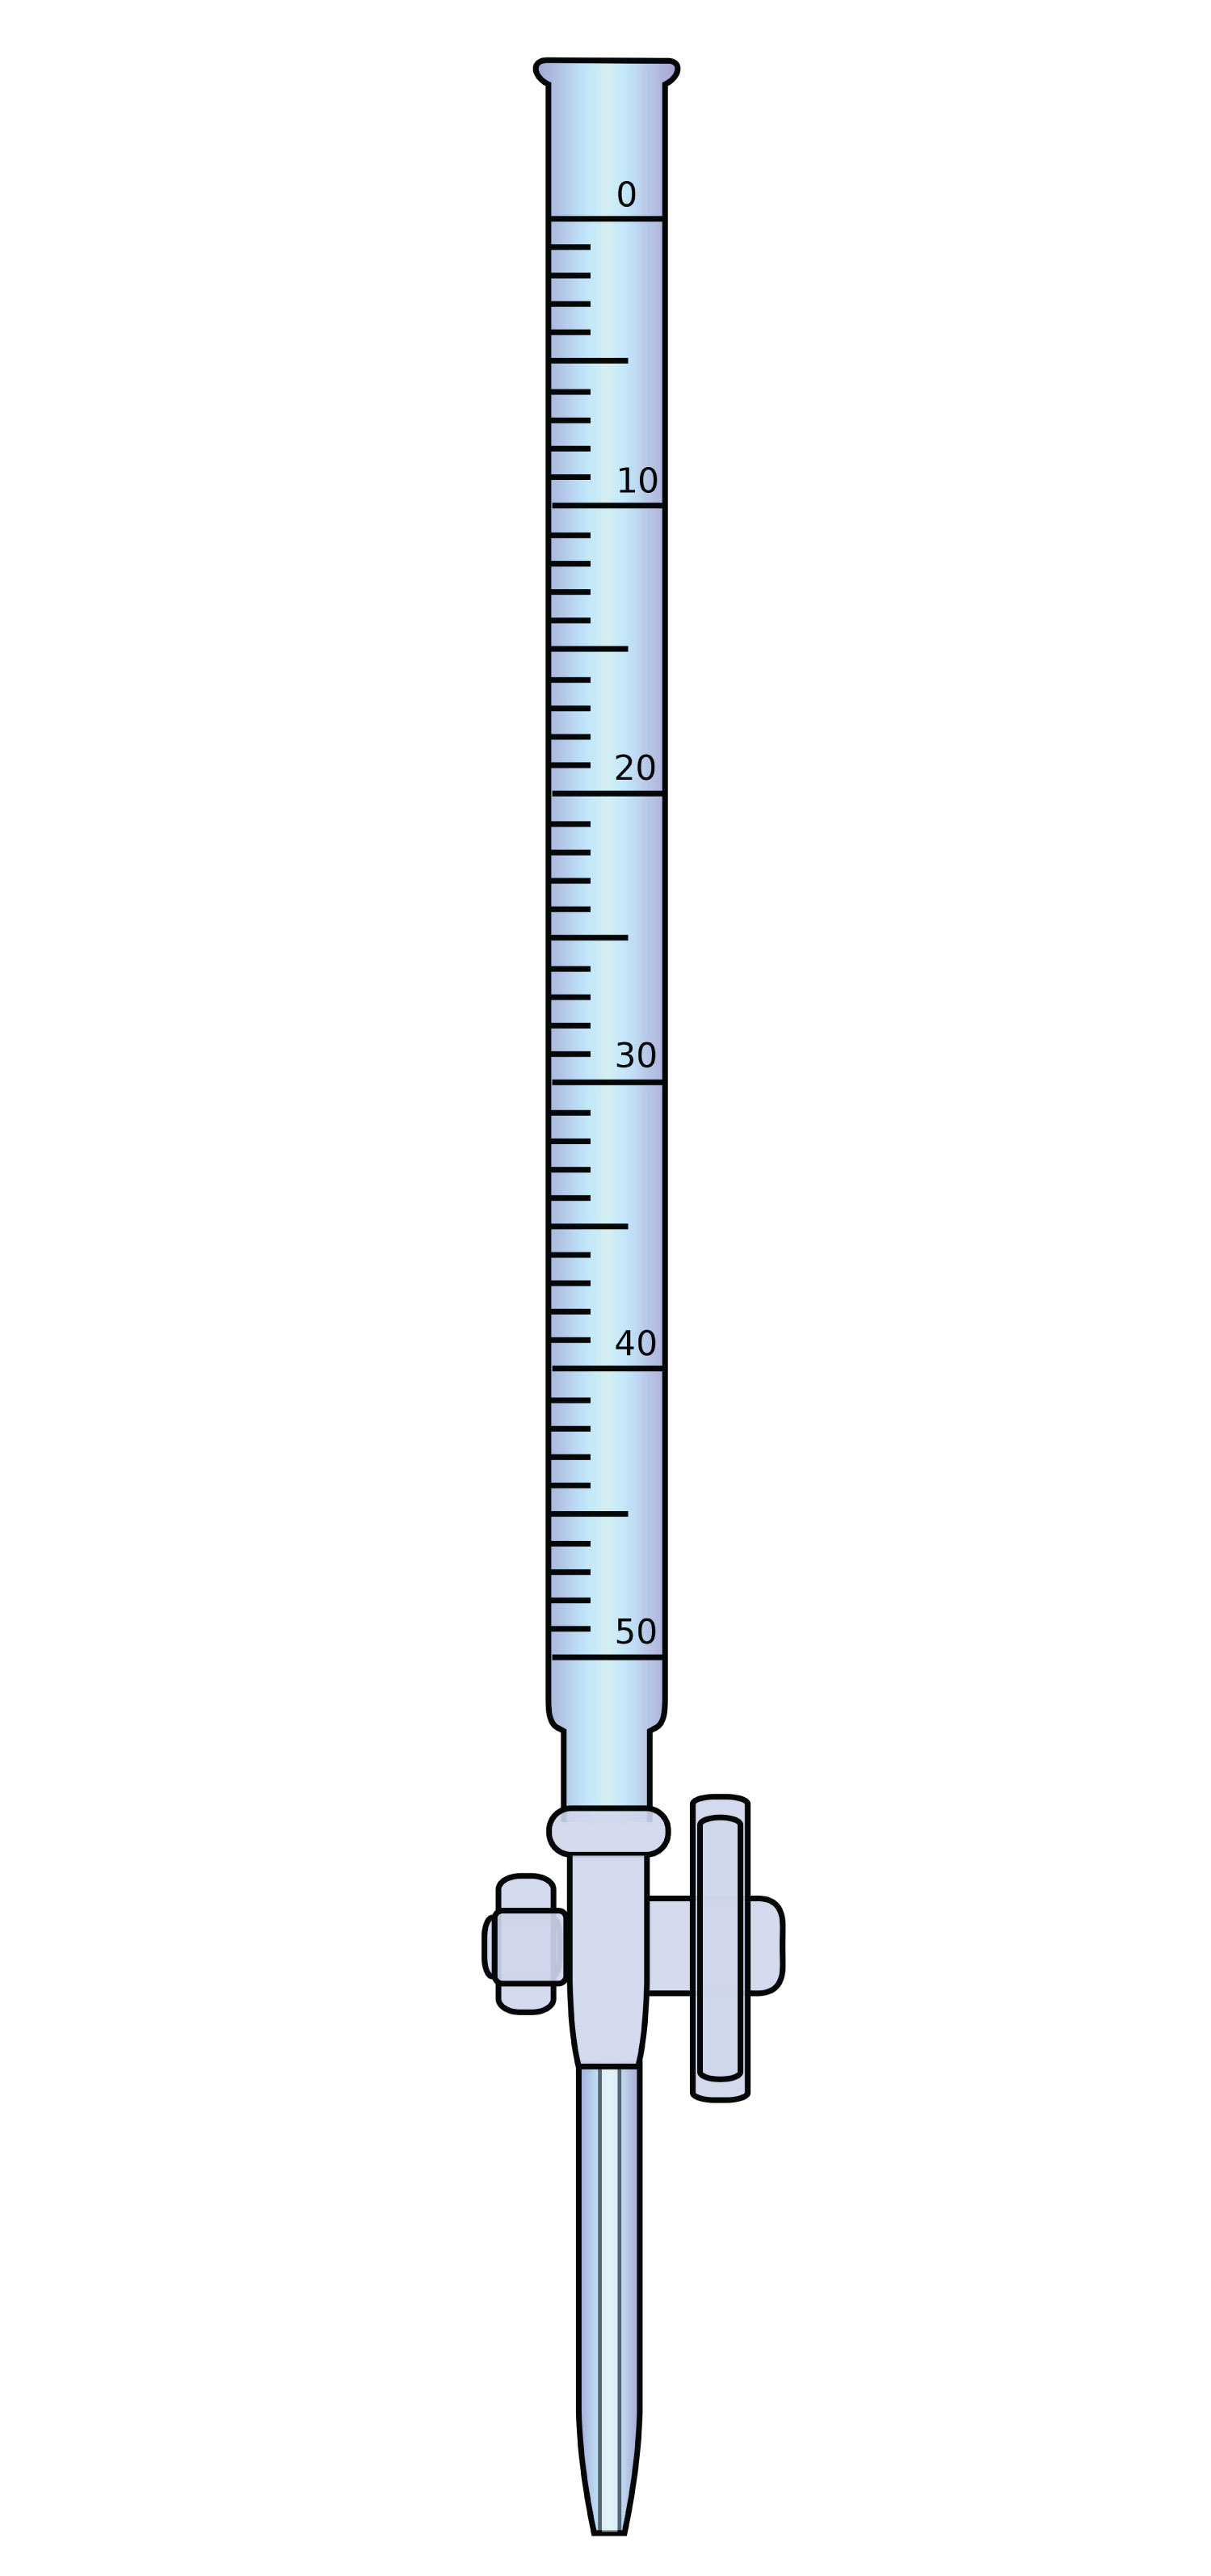
\includegraphics[scale =
0.05]{buret} \captionof{figure}{Illustration of burette. \cite{buret}}
\end{center} The burette is usually glass so that the liquid inside can be
observed easily. The numbers on a burette are labled "backwards", with "0" at
the top and increasing as they proceed down the side. In this manner, it is easy
to measure the amount of titrant used by subtracting the final volume remaining
in the burette from the initial volume. There is a valve at the bottom of the
burette that allows the titrant to be released ranging from a steady flow to a
single drop. Controlling the level of flow is essential in ensuring that an
accurate measurement of titrant needed for the reaction to proceed to completion
is taken.

\subsection {Using a pH Meter}
An acidic solution contains more postively charged hydrogen ions than an
alkaline solution, therefore it has a greater potentional to produce an
electrical current given the correct situations. A pH meter is able to measure
the pH of a solution by measuring and comparing the electrical potential that is produced by
the solution with the voltage of a reference solution. 

A pH meter consist of two parts, the meter itself and two electrodes (in this
lab, both electrodes are contained within a single probe). The glass electrode
consists of an electrical wire in a solution of potassium chloride, contained
within a small glass bulb containing metal salts. The second electrode, known as
the reference electrode, consists of a potassium chloride wire in a solution of
potassium chloride. Figure 2 illustrates the various parts of a pH meter.
\cite{meter}

\begin{center}
        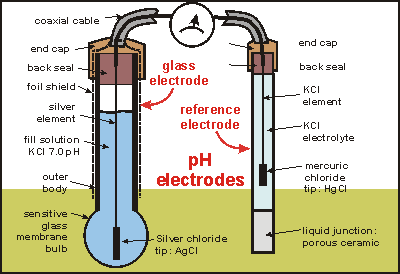
\includegraphics[scale=0.6]{meter}
        \captionof{figure}{Diagram of a pH meter. \cite{meter}}
\end{center}

Upon insertion of the probe into a solution, an ion exchange process occurs
between the hydrogen ions in solution and the metal ions on the outer surface of
the glass electrode. A secondary ion exchange also occurs on the inside surface
of the glass electrode.  As a result of the two solutions on either side of the
glass having different levels of acidity, a different level of ion exchange
occurs on the two sides.  This difference creates an electrical charge specific
to the potential difference and the meter is able to register a difference in
voltage between the two electrodes. The voltage produced is proportional to the
logarithm of the hydrogen ion activity, as given by the Nernst equation.
\cite{electrode}

This method of calculating the pH of a solution based on differences in hydrogen
ion activity requires the pH meter to be properly calibrated in order to be
accurate. A pH meter can be calibrated by using a reference solution, or buffer,
of a known pH. It is important to note that this method of calibration requires
that temperature remain constant. 

\newpage


\section {Results and Discussion}

All graphs were generated through Matlab and through the use of numerical
methods.
Figure 3 shows the graphs of the pH measurements made vs. the amount of NaOH
added. The areas with the steepest slopes correspond with the end points of the
titration.
\begin{center}
        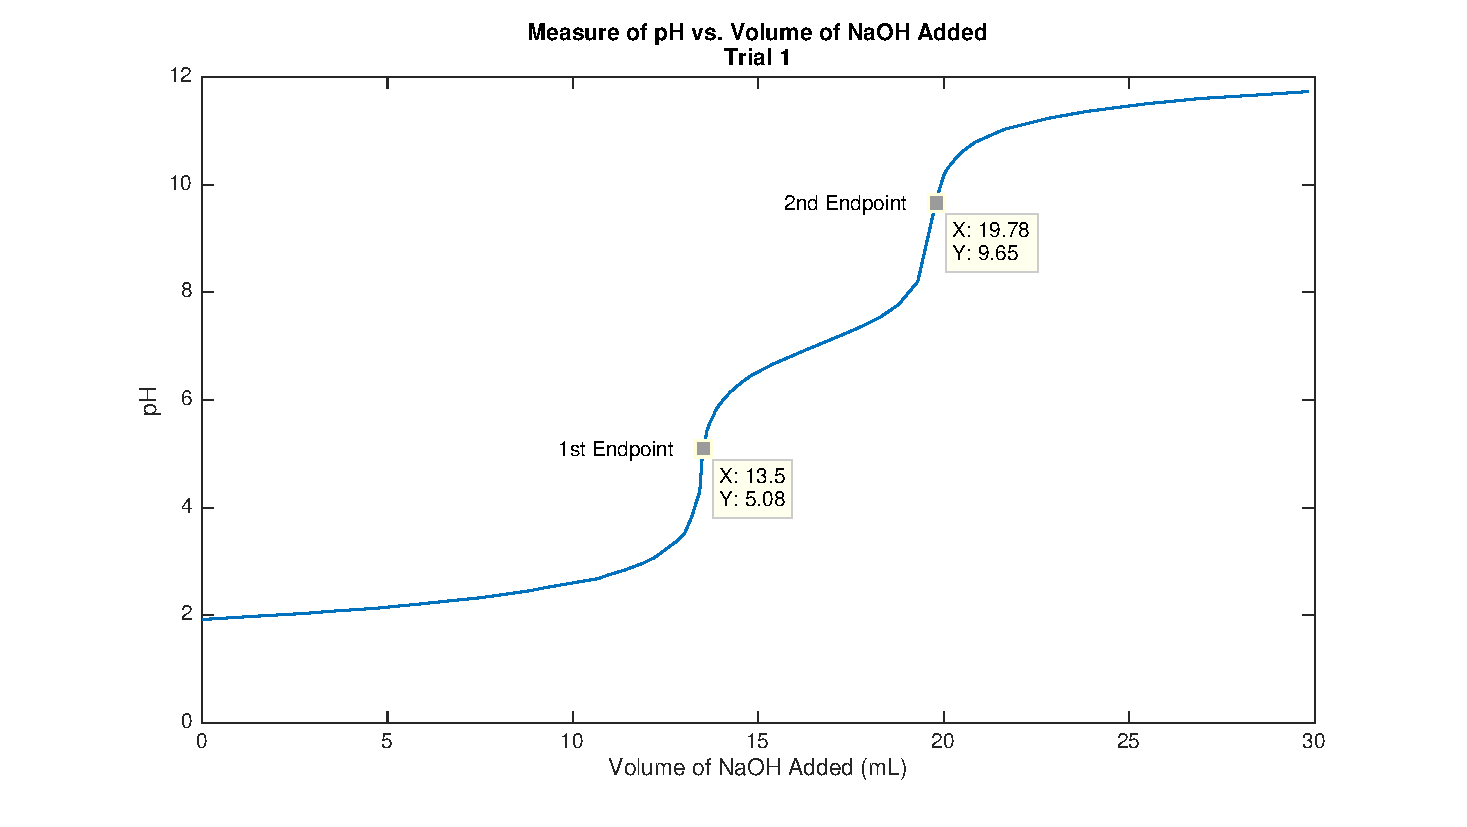
\includegraphics[scale=0.7]{raw_1}
        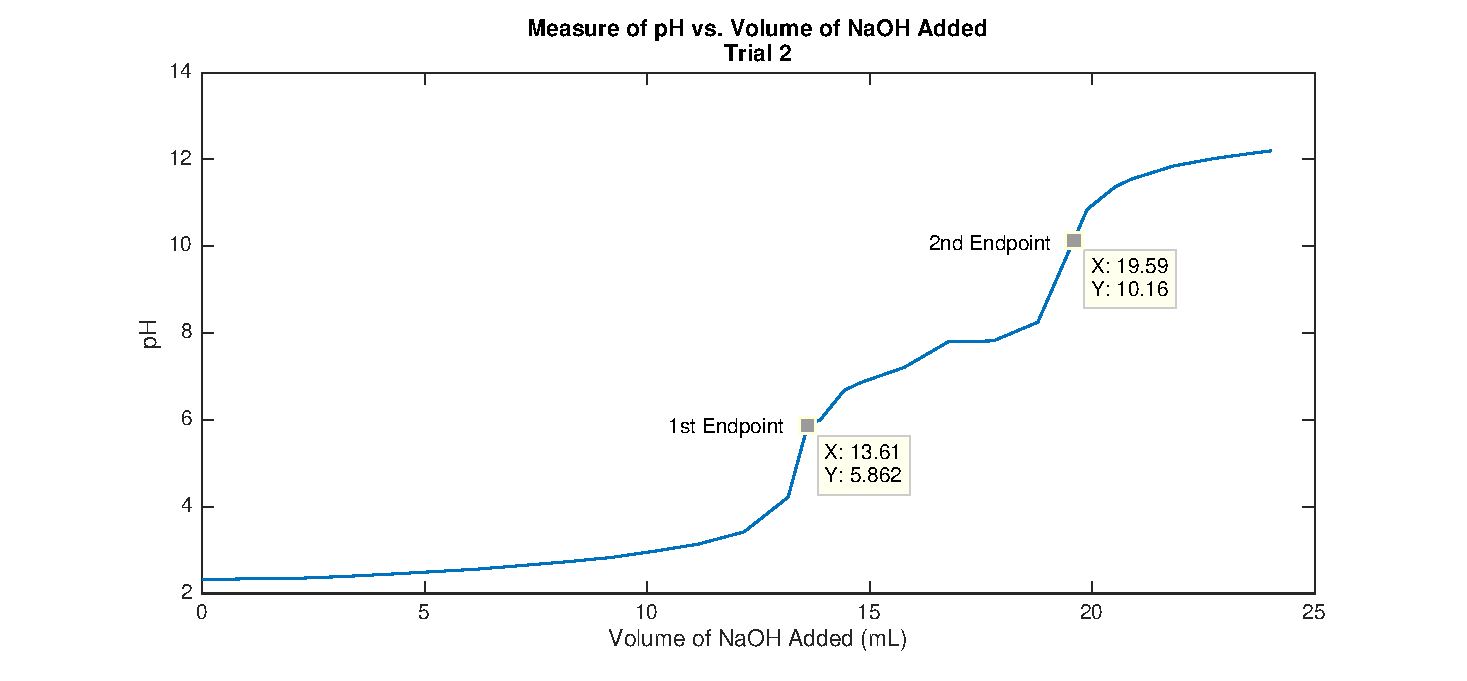
\includegraphics[scale=0.7]{raw_2}
        \captionof{figure}{Raw data of pH vs. amount of NaOH added for both
        trials.}
\end{center}
\newpage

Figure 4 shows the graphs of the first derivatives of pH vs. amount of NaOH
added. The local maxima correspond with the end points of the titration.
\begin{center}
        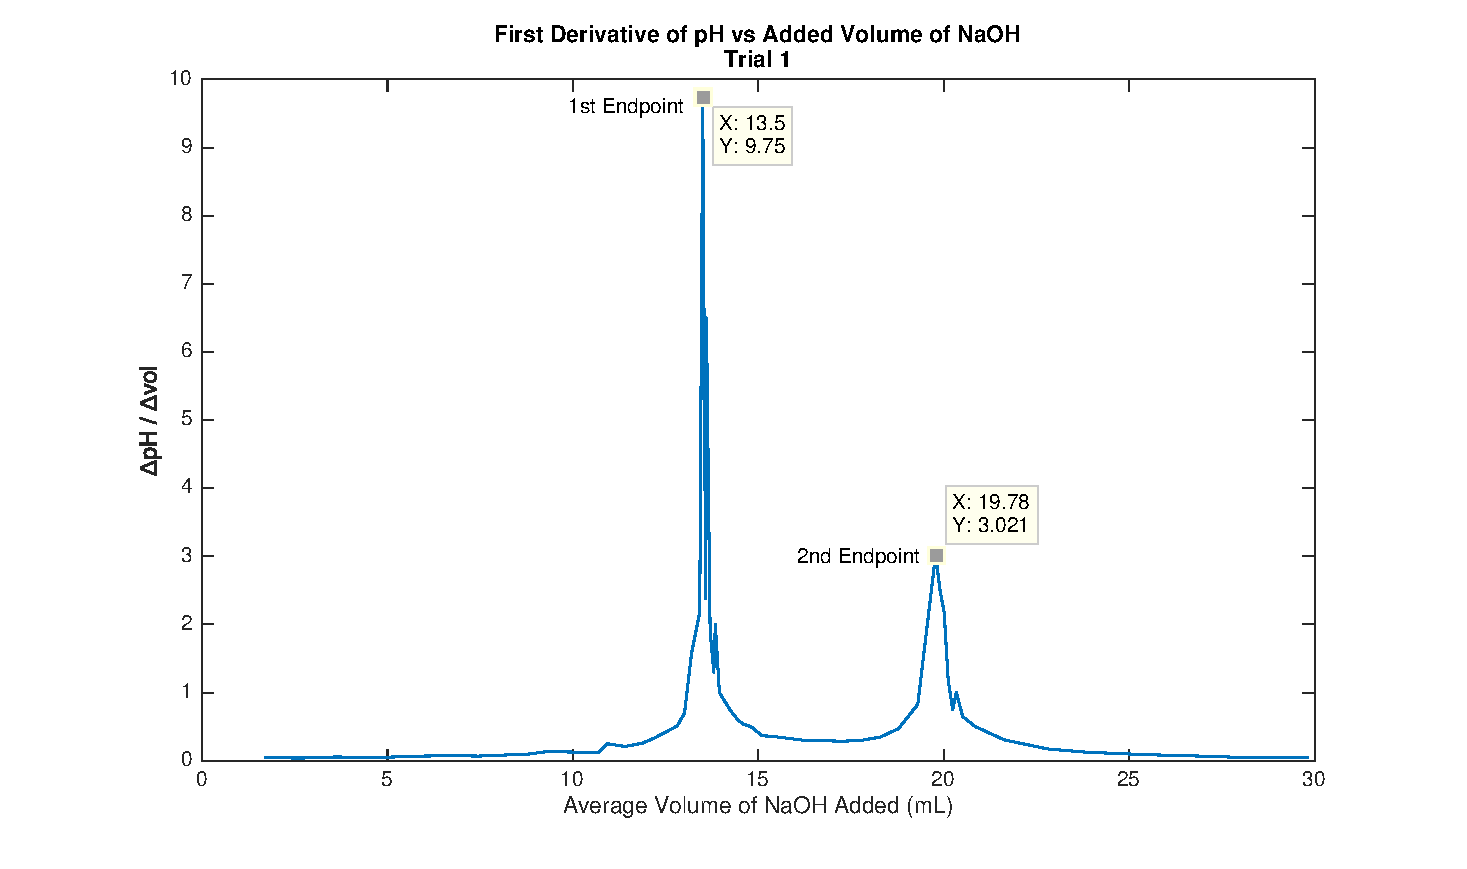
\includegraphics[scale=0.7]{1dev_1}
        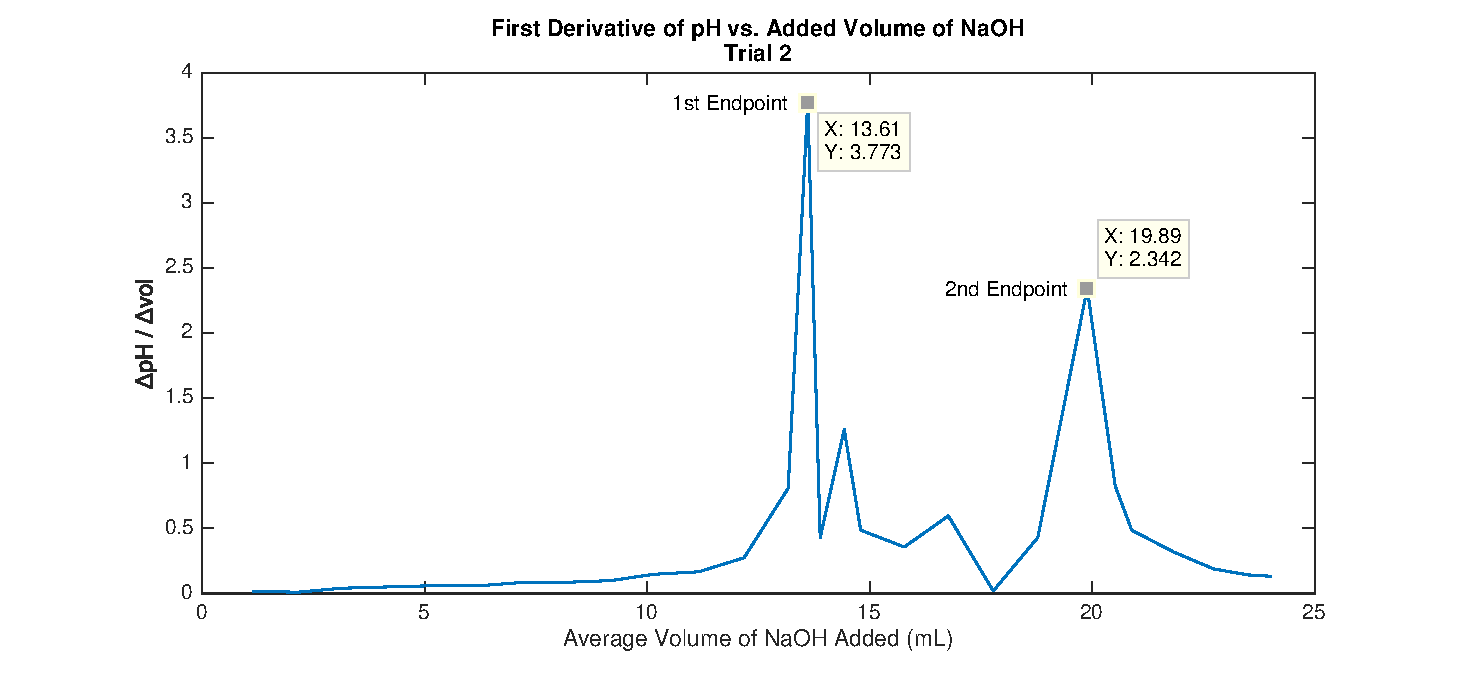
\includegraphics[scale=0.7]{1dev_2}
        \captionof{figure}{First derivative of pH vs. amount of NaOH added for both
        trials.}
\end{center}
\newpage

Figure 5 shows the graphs of the second derivatives of pH vs. amount of NaOH
added. The X-intercepts correspond with the end points of the titration.
\begin{center}
        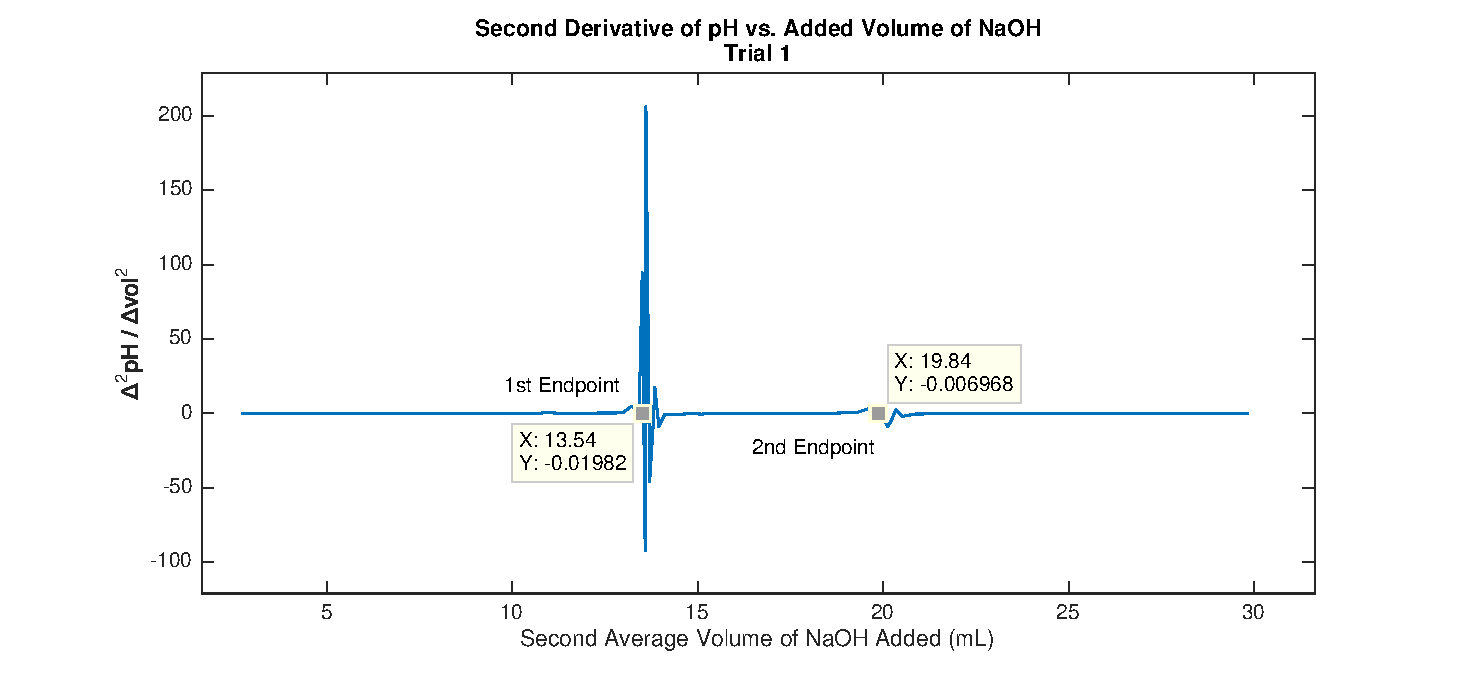
\includegraphics[scale=0.7]{2dev_1}
        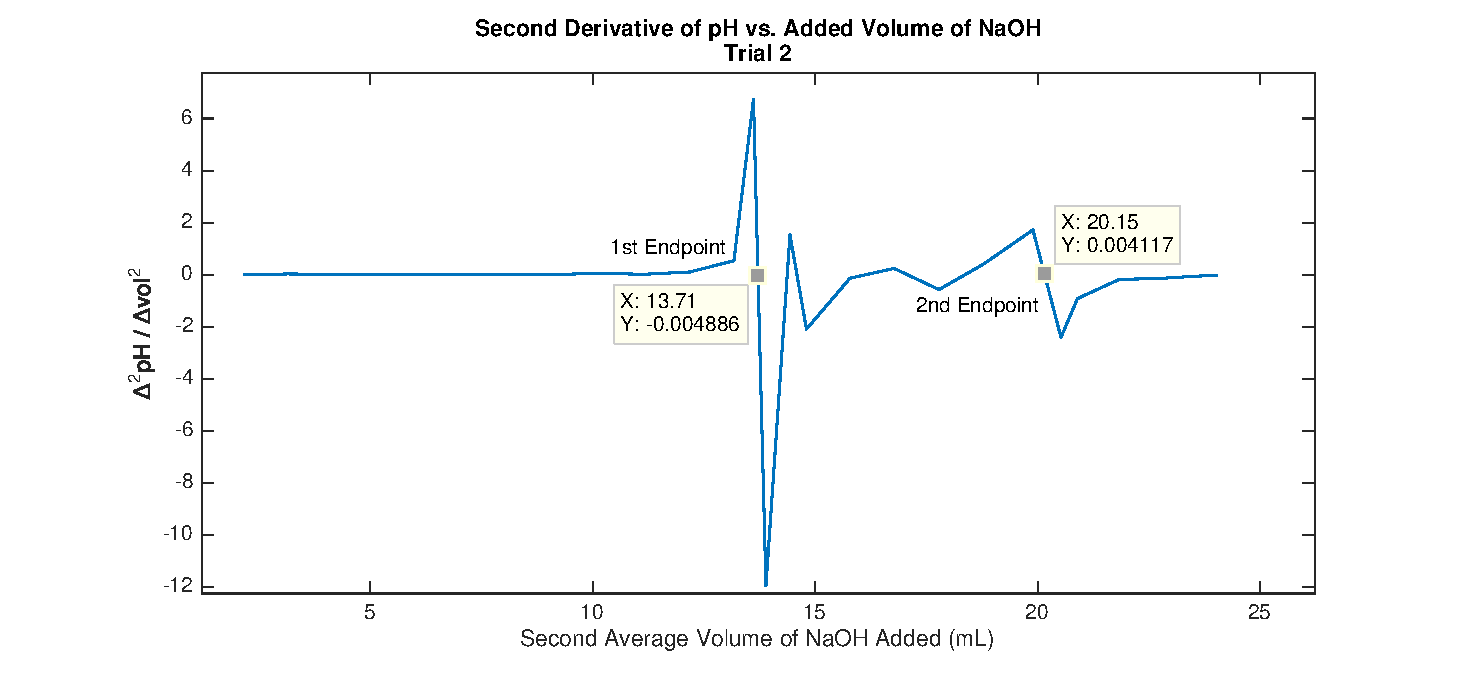
\includegraphics[scale=0.7]{2dev_2}
        \captionof{figure}{Second derivative of pH vs. amount of NaOH added for both
        trials.}
\end{center}
\newpage

Figure 6 shows the graphs of the second derivatives of the first endpoint of pH vs. amount of NaOH
added.
\begin{center}
        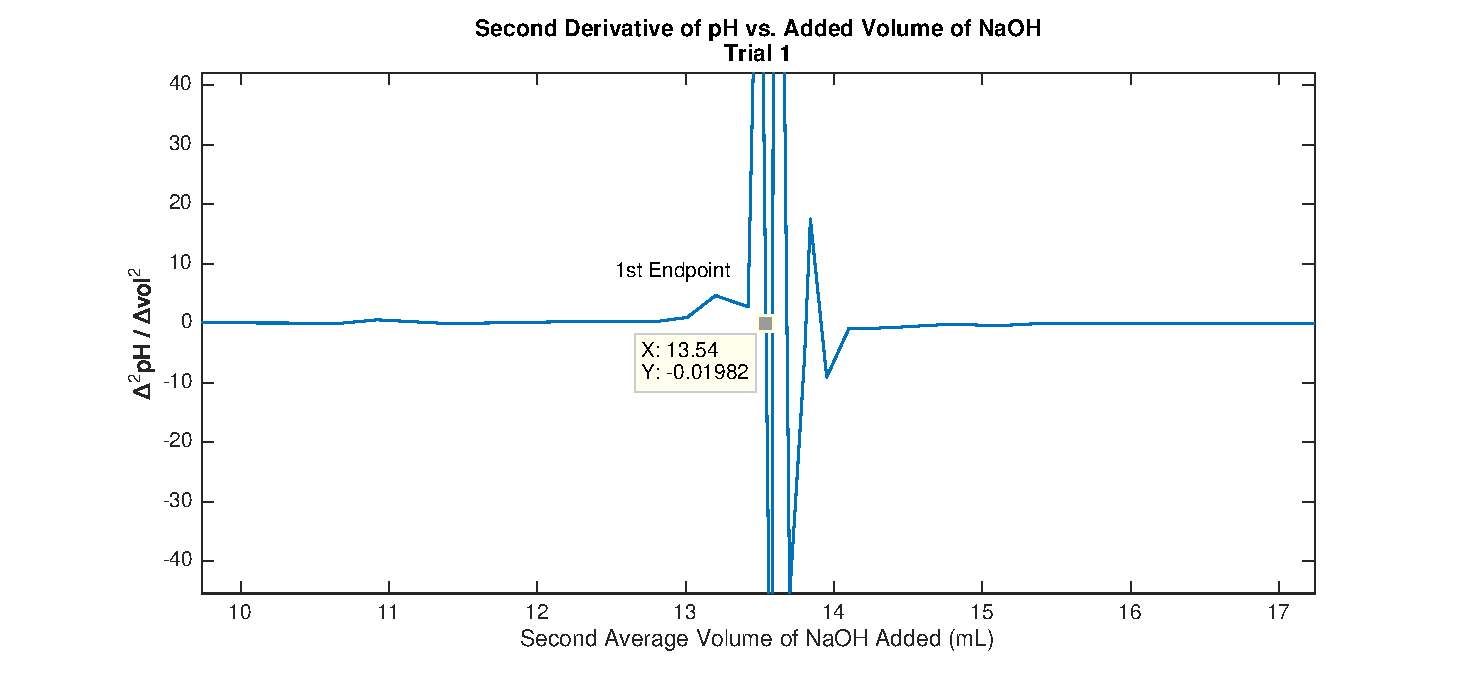
\includegraphics[scale=0.7]{2dev_1_1}
        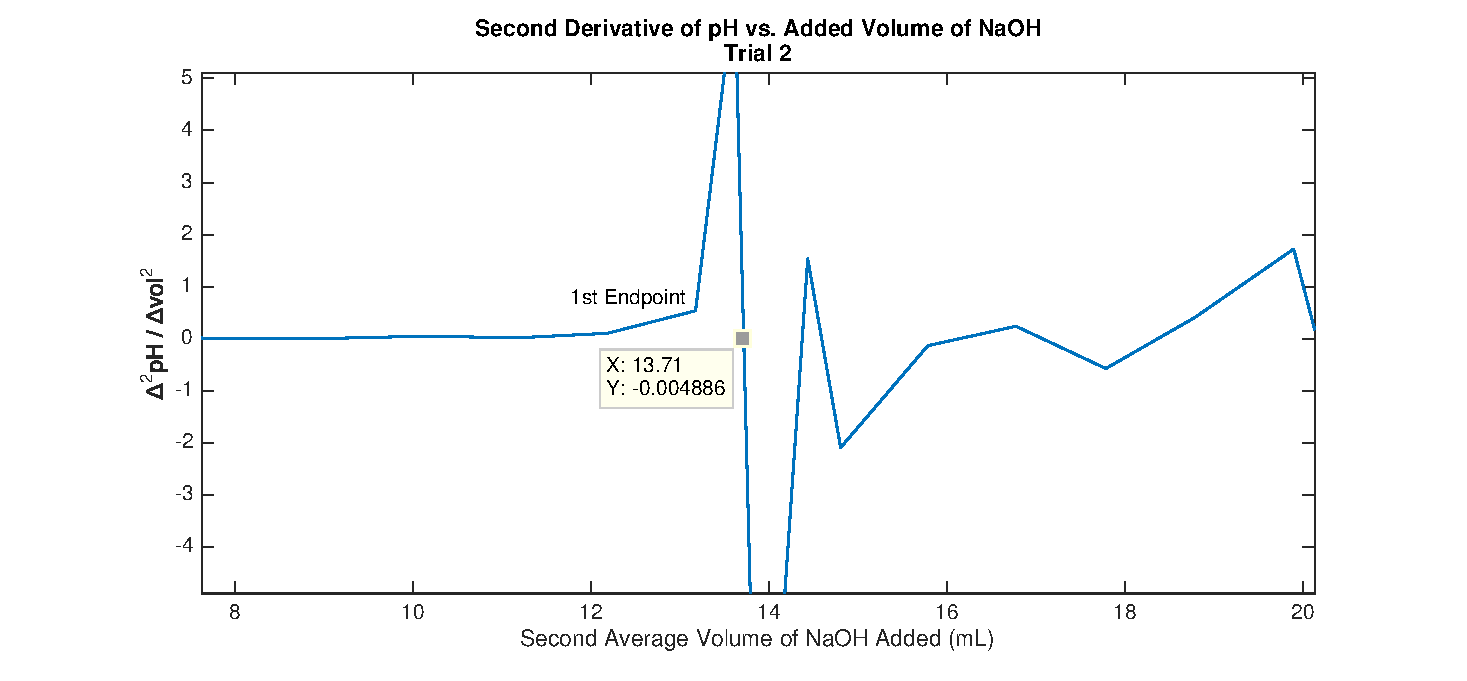
\includegraphics[scale=0.7]{2dev_1_2}
        \captionof{figure}{Second derivative of first endpoint of pH vs. amount of NaOH added for both
        trials.}
\end{center}
\newpage 

Figure 7 shows the graphs of the second derivatives of the second endpoint of pH vs. amount of NaOH
added. 
\begin{center}
        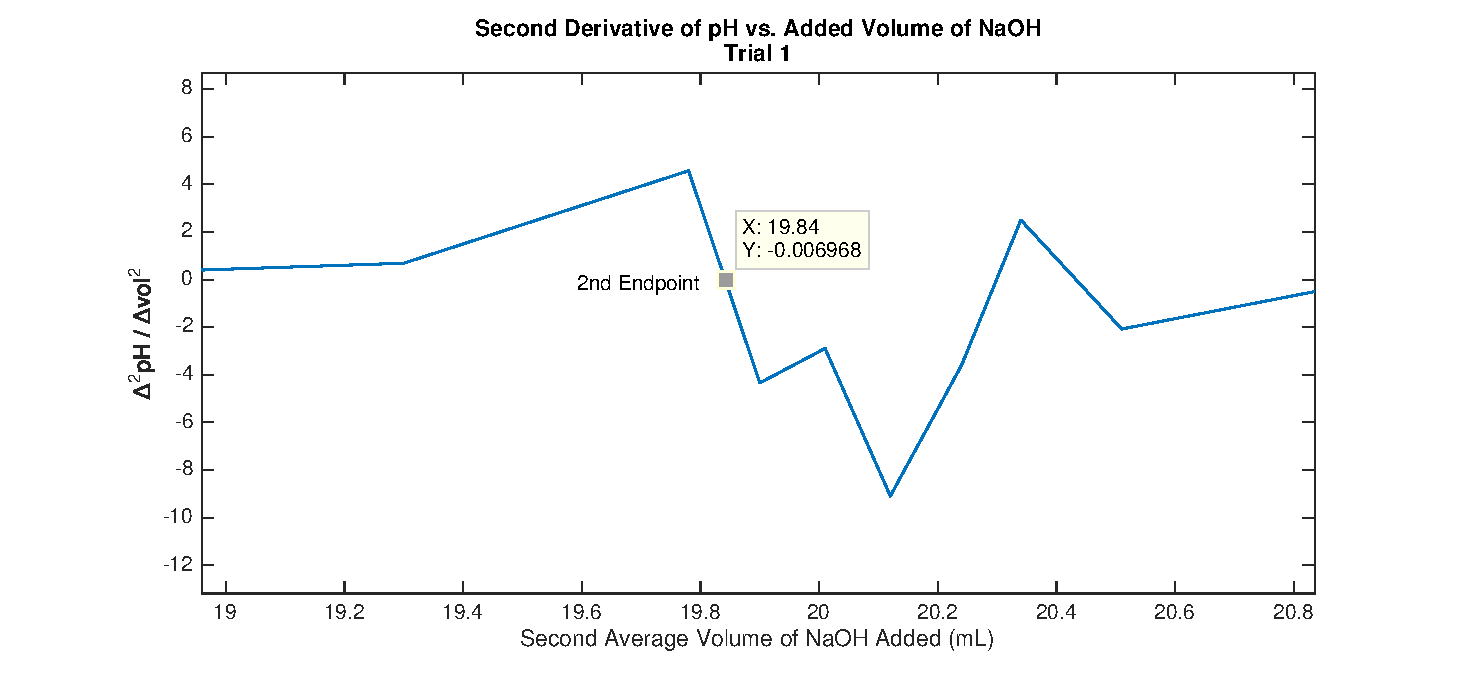
\includegraphics[scale=0.7]{2dev_2_1}
        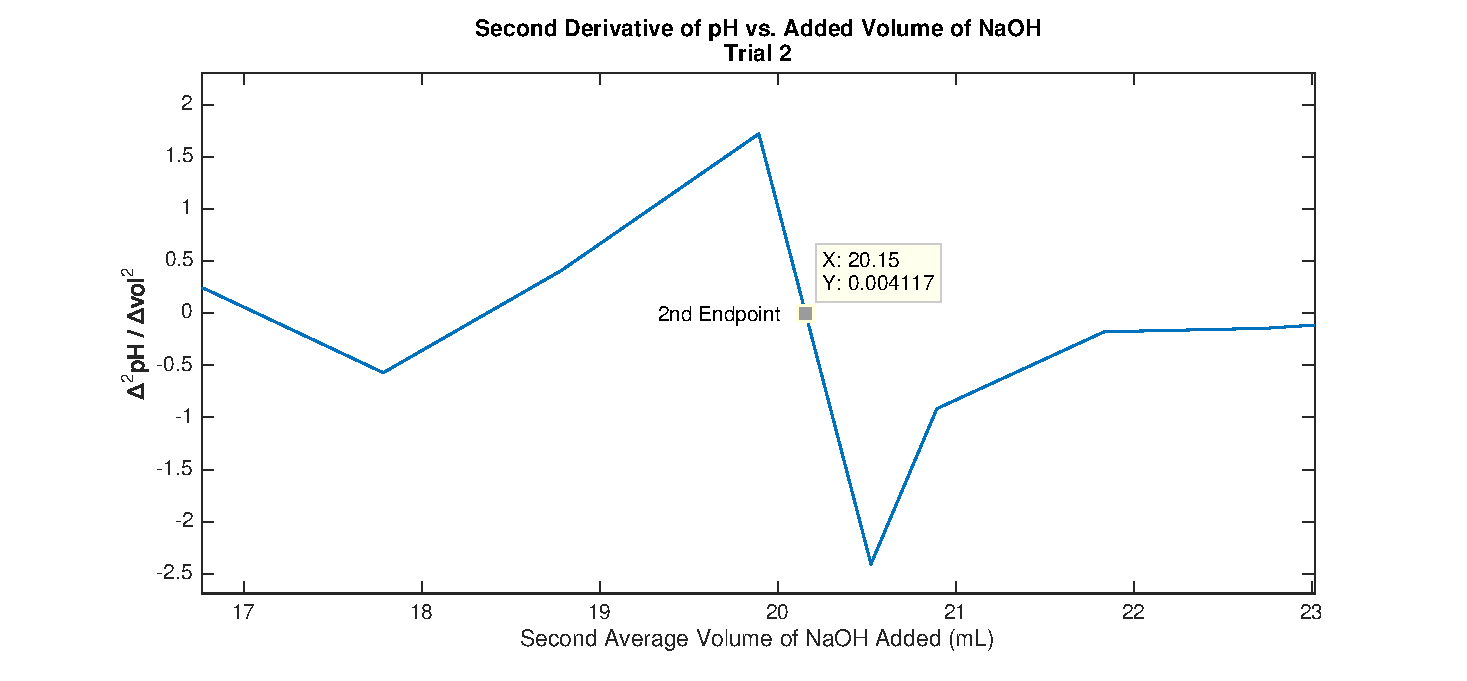
\includegraphics[scale=0.7]{2dev_2_2}
        \captionof{figure}{Second derivative of second endpoint pH vs. amount of NaOH added for both
        trials.}
\end{center}

Please refer to the Appendix for detailed calculations in determining results.

The graphs of the second derivatives were used in accurately determining the
end points for the titrations. An average was taken between the two trials and
the concentrations of HCl and H$_3$PO$_4$ were determined to be 0.0272 M and
0.0238 M respectively in Unknown solution 7.
Table 1 summarizes these results.
\begin{center}
\begin{tabular}{|c|c|}
        \hline
        & Average \\
        \hline
        HCl concentration & 0.0272 M \\
        \hline
        H$_3$PO$_4$ concentration & 0.0238 M \\
        \hline
\end{tabular}
        \captionof{table}{Determined concentrations of acidic species in unknown
        solution 7.}
\end{center}

Improvements that could be made to increase the accuracy and precision of this
experiment may include the inclusion of more trials.


\section {Conclusion}

The concentrations of an unknown mixture of HCl and H$_3$PO$_4$ were determined
to be 0.0272 M and 0.0238 M respectively through potentiometric titration. These
values are expected to be reasonably accurate based on the concentration of NaOH
that was used as a titrant (which was 0.09357 M).  Sources of error may include
systematic error in the use of the pH meters.  Mis-calibration, or even a
differing of calibration methods, of pH meters will result in different results
and conclusions.


\newpage
\bibliographystyle{unsrt}
\bibliography{poten.bib}
\newpage

\section*{Appendix}

\begin{enumerate}
        \item Tabular data used to generate graphs.
        \item Lab notebook pages with raw data and calculations.
\end{enumerate}

\end {document}
